\section{Physics Applications:  Work, Force, and Pressure} \label{S:6.5.Physics}

\begin{goals}
  \item How do we measure the work accomplished by a varying force that moves an object a certain distance?
  \item What is the total force exerted by water against a dam?
  \item How are both of the above concepts and their corresponding use of definite integrals similar to problems we have encountered in the past involving formulas such as ``distance equals rate times time'' and ``mass equals density times volume''?
\end{goals}

%-----------------------------------
% SUBSECTION INTRODUCTION
%-----------------------------------
\subsection*{Introduction}

%\begin{figure*}[h]
%\begin{flushleft}
%\includegraphics{figures/6_4_Intro.eps}
%\caption{Three settings where we compute the accumulation of a varying quantity:  the area under $y = f(x)$, the distance traveled by an object with velocity $y = v(t)$, and the mass of a bar with density function $y=\rho(x)$.} 
%\label{F:6.4.Intro}
%\end{flushleft}
%\end{figure*}

In our work to date with the definite integral, we have seen several different circumstances where the integral enables us to measure the accumulation of a quantity that varies, provided the quantity is approximately constant over small intervals.  For instance, based on the fact that the area of a rectangle is $A = l \cdot w$, if we wish to find the area bounded by a nonnegative curve $y = f(x)$ and the $x$-axis on an interval $[a,b]$, a representative slice of width $\triangle x$ has  area $A_{\mbox{\small{slice}}} = f(x) \triangle x$, and thus as we let the width of the representative slice tend to zero, we find that the exact area of the region is
$$A = \int_a^b f(x) \, dx.$$
In a similar way, if we know that the velocity of a moving object is given by the function $y = v(t)$, and we wish to know the distance the object travels on an interval $[a,b]$ where $v(t)$ is nonnegative, we can use a definite integral to generalize the fact that $d = r \cdot t$ when the rate, $r$, is constant.  More specifically, on a short time interval $\triangle t$, $v(t)$ is roughly constant, and hence for a small slice of time, $d_{\mbox{\small{slice}}} = v(t) \triangle t$, and so as the width of the time interval $\triangle t$ tends to zero, the exact distance traveled is given by the definite integral
$$d = \int_a^b v(t) \, dt.$$
Finally, when we recently learned about the mass of an object of non-constant density, we saw that since $M = D \cdot V$ (mass equals density times volume, provided that density is constant), if we can consider a small slice of an object on which the density is approximately constant, a definite integral may be used to determine the exact mass of the object.  For instance, if we have a thin rod whose cross sections have constant density, but whose density is distributed along the $x$ axis according to the function $y = \rho(x)$, it follows that for a small slice of the rod that is $\triangle x$ thick, $M_{\mbox{\small{slice}}} = \rho(x) \triangle x$.  In the limit as $\triangle x \to 0$, we then find that the total mass is given by 
$$M = \int_a^b \rho(x) \, dx.$$

Note that all three of these situations are similar in that we have a basic rule ($A = l \cdot w$, $d = r \cdot t$, $M = D \cdot V$) where one of the two quantities being multiplied is no longer constant; in each, we consider a small interval for the other variable in the formula, calculate the approximate value of the desired quantity (area, distance, or mass) over the small interval, and then use a definite integral to sum the results as the length of the small intervals is allowed to approach zero.  It should be apparent that this approach will work effectively for other situations where we have a quantity of interest that varies.  

We next turn to the notion of \emph{work}\index{work}:  from physics, a basic principal is that work is the product of force and distance.  For example, if a person exerts a force of 20 pounds to lift a 20-pound weight 4 feet off the ground, the total work accomplished is
$$W = F \cdot d = 20 \cdot 4 = 80 \ \mbox{foot-pounds}.$$
If force and distance are measured in English units (pounds and feet), then the units on work are \emph{foot-pounds}\index{foot-pound}.  If instead we work in metric units, where forces are measured in Newtons and distances in meters, the units on work are \emph{Newton-meters}\index{Newton-meter}.

Of course, the formula $W = F \cdot d$ only applies when the force  is constant while it is exerted over the distance $d$.  In Preview Activity~\ref{PA:6.5}, we explore one way that we can use a definite integral to compute the total work accomplished when the force exerted varies.

\input{previews/6.5.PA1} % PREVIEW ACTIVITY

%--------------------------
% SUBSECTION WORK
%-------------------------
\subsection*{Work} \index{work}

Because work is calculated by the rule $W = F \cdot d$, whenever the force $F$ is constant, it follows that we can use a definite integral to compute the work accomplished by a varying force.  For example, suppose that in a setting similar to the problem posed in Preview Activity~\ref{PA:6.5}, we have a bucket being lifted in a $50$-foot well whose weight at height $h$ is given by $B(h) = 12 + 8e^{-0.1h}$.  

In contrast to the problem in the preview activity, this bucket is not leaking at a constant rate; but because the weight of the bucket and water is not constant, we have to use a definite integral to determine the total work that results from lifting the bucket.  Observe that at a height $h$ above the water, the approximate work to move the bucket a small distance $\triangle h$ is
$$W_{\mbox{\small{slice}}} = B(h) \triangle h = (12 + 8e^{-0.1h}) \triangle h.$$
Hence, if we let $\triangle h$ tend to $0$ and take the sum of all of the slices of work accomplished on these small intervals, it follows that the total work is given by
$$W = \int_0^{50} B(h) \, dh = \int_0^{50} (12 + 8e^{-0.1h}) \, dh.$$
While is a straightforward exercise to evaluate this integral exactly using the Fundamental Theorem of Calculus, in applied settings such as this one we will typically use computing technology to find accurate approximations of integrals that are of interest to us.  Here, it turns out that $W = \int_0^{50} (12 + 8e^{-0.1h}) \, dh \approx 679.461$ foot-pounds.

Our work in the most recent example above employs the following important general principle.

\concept{Work}{ % CONCEPT
For an object being moved in the positive direction along an axis, $x$, by a force $F(x)$, the total work to move the object from $a$ to $b$ is given by
$$W = \int_a^b F(x) \, dx.$$
} % end concept

%\begin{marginfigure} % MARGIN FIGURE
%\margingraphics{figures/6_4_DamEx.eps}
%\caption{A trapezoidal dam that is 25 feet tall, 60 feet wide at its base, 90 feet wide at its top, with the water line 5 feet down from the top of its face.} \label{F:6.4.DamEx}
%\end{marginfigure}

\begin{example} \label{eg:6.5.2} % EXAMPLE
How much work is performed pulling a 60 m climbing rope up a cliff face, where the rope has a mass of 66 g/m?


\solution We need to create a force function $F(x)$ on the interval $[0,60]$. To do so, we must first decide what $x$ is measuring: it is the length of the rope still hanging or is it the amount of rope pulled in? As long as we are consistent, either approach is fine. We adopt for this example the convention that $x$ is the amount of rope pulled in. This seems to match intuition better; pulling up the first 10 meters of rope involves $x=0$ to $x=10$ instead of $x=60$ to $x=50$. 

As $x$ is the amount of rope pulled in, the amount of rope still hanging is $60-x$. This length of rope has a mass of 66 g/m, or $0.066$ kg/m. The the mass of the rope still hanging is $0.066(60-x)$ kg; multiplying this mass by the acceleration of gravity, 9.8 m/s$^2$, gives our variable force function $$F(x) = (9.8)(0.066)(60-x) = 0.6468(60-x).$$

Thus the total work performed in pulling up the rope is 
$$W = \int_0^{60} 0.6468(60-x)\ dx = 1,164.24\ \text{J}.$$

By comparison, consider the work done in lifting the entire rope 60 meters. The rope weights $60\times 0.066 \times 9.8 = 38.808$ N, so the work applying this force for 60 meters is $60\times 38.808 = 2,328.48$ J. This is exactly twice the work calculated before (and we leave it to the reader to understand why.)
\end{example} % EXAMPLE

%\begin{marginfigure} % MARGIN FIGURE
%\margingraphics{figures/6_4_DamEx.eps}
%\caption{A trapezoidal dam that is 25 feet tall, 60 feet wide at its base, 90 feet wide at its top, with the water line 5 feet down from the top of its face.} \label{F:6.4.DamEx}
%\end{marginfigure}

\begin{example} \label{eg:6.5.3} % EXAMPLE
A box of 100 lb of sand is being pulled up at a uniform rate a distance of 50 ft over 1 minute. The sand is leaking from the box at a rate of 1 lb/s. The box itself weighs 5 lb and is pulled by a rope weighing .2 lb/ft. 
	\begin{enumerate}
	\item		How much work is done lifting just the rope?
	\item		How much work is done lifting just the box and sand?
	\item		What is the total amount of work performed?
	\end{enumerate}

\solution
\begin{enumerate}
	\item		We start by forming the force function $F_r(x)$ for the rope (where the subscript denotes we are considering the rope). As in the previous example, let $x$ denote the amount of rope, in feet, pulled in. (This is the same as saying $x$ denotes the height of the box.) The weight of the rope with $x$ feet pulled in is $F_r(x) = 0.2(50-x) = 10-0.2x$. (Note that we do not have to include the acceleration of gravity here, for the \textit{weight} of the rope per foot is given, not its \textit{mass} per meter as before.) The work performed lifting the rope is 
	$$W_r = \int_0^{50} (10-0.2x)\ dx = 250\ \text{ft--lb}.$$
	
	\item	The sand is leaving the box at a rate of 1 lb/s. As the vertical trip is to take one minute, we know that 60 lb will have left when the box reaches its final height of 50 ft. Again letting $x$ represent the height of the box, we have two points on the line that describes the weight of the sand: when $x=0$, the sand weight is 100 lb, producing the point $(0,100)$; when $x=50$, the sand in the box weighs 40 lb, producing the point $(50,40)$. The slope of this line is $\frac{100-40}{0-50} = -1.2$, giving the equation of the weight of the sand at height $x$ as $w(x) = -1.2x+100$. The box itself weighs a constant 5 lb, so the total force function is $F_b(x) = -1.2x+105$. Integrating from $x=0$ to $x=50$ gives the work performed in lifting box and sand:
	$$W_b = \int_0^{50} (-1.2x+105)\ dx = 3750\ \text{ft--lb.}$$
	
	\item	The total work is the sum of $W_r$ and $W_b$: $250+3750=4000$ ft--lb. We can also arrive at this via integration:
	\begin{align*} W &= \int_0^{50} (F_r(x)+F_b(x))\ dx \\
									&= \int_0^{50} (10-0.2x-1.2x+105)\ dx \\
									&= \int_0^{50} (-1.4x+115) \ dx \\
									&= 4000 \ \text{ft--lb.}
	\end{align*}	
\end{enumerate}

\end{example} % EXAMPLE

%\begin{marginfigure} % MARGIN FIGURE
%\margingraphics{figures/ex_spring1}
%\caption{Illustrating the important aspects of stretching a spring in computing work in Example \ref{eg:6.5.4}.} \label{F:6.4.HookeEx}
%\end{marginfigure}

\begin{example} \label{eg:6.5.4} % EXAMPLE
Hooke's Law states that the force required to compress or stretch a spring $x$ units from its natural length is proportional to $x$; that is, this force is $F(x) = kx$ for some constant $k$.

A force of 20 lb stretches a spring from a length of 7 inches to a length of 12 inches. How much work was performed in stretching the spring to this length?

\solution
In many ways, we are not at all concerned with the actual length of the spring, only with the amount of its change. Hence, we do not care that 20 lb of force stretches the spring to a length of 12 inches, but rather that a force of 20 lb stretches the spring by 5 in. This is illustrated in Figure \ref{F:6.4.HookeEx}; we only measure the change in the spring's length, not the overall length of the spring.

Converting the units of length to feet, we have $$F(5/12) = 5/12k = 20\ \text{lb}.$$ Thus $k = 48$ lb/ft and $F(x) = 48x$. 

We compute the total work performed by integrating $F(x)$ from $x=0$ to $x=5/12$:
\begin{align*}
W 	&= 	\int_0^{5/12} 48x \ dx \\
&=	24x^2\Big|_0^{5/12} \\
&=  25/6 \approx 4.1667\ \text{ft--lb.}
\end{align*}

\end{example} % EXAMPLE

\begin{activity} \label{A:6.5.1}  Consider the following situations in which a varying force accomplishes work.
\ba
	\item Suppose that a heavy rope hangs over the side of a cliff.  The rope is 200 feet long and weighs 0.3 pounds per foot; initially the rope is fully extended.  How much work is required to haul in the entire length of the rope?  (Hint: set up a function $F(h)$ whose value is the weight of the rope remaining over the cliff after $h$ feet have been hauled in.)
	\item A leaky bucket is being hauled up from a 100 foot deep well.  When lifted from the water, the bucket and water together weigh 40 pounds.  As the bucket is being hauled upward at a constant rate, the bucket leaks water at a constant rate so that it is losing weight at a rate of 0.1 pounds per foot.  What function $B(h)$ tells the weight of the bucket after the bucket has been lifted $h$ feet?  What is the total amount of work accomplished in lifting the bucket to the top of the well?
	\item Now suppose that the bucket in (b) does not leak at a constant rate, but rather that its weight at a height $h$ feet above the water is given by $B(h) = 25 + 15e^{-0.05h}$.  What is the total work required to lift the bucket 100 feet?  What is the average force exerted on the bucket on the interval $h = 0$ to $h = 100$?
	\item From physics, \emph{Hooke's Law} \index{Hooke's Law} for springs states that the amount of force required to hold a spring that is compressed (or extended) to a particular length is proportionate to the distance the spring is compressed (or extended) from its natural length.  That is, the force to compress (or extend) a spring $x$ units from its natural length is $F(x) = kx$ for some constant $k$ (which is called the \emph{spring constant}.) For springs, we choose to measure the force in pounds and the distance the spring is compressed in feet.
	
	Suppose that a force of 5 pounds extends a particular spring 4 inches (1/3 foot) beyond its natural length.
	\be
		\item[i.]  Use the given fact that $F(1/3) = 5$ to find the spring constant $k$.
		\item[ii.]  Find the work done to extend the spring from its natural length to 1 foot beyond its natural length.
		\item[iii.]  Find the work required to extend the spring from 1 foot beyond its natural length to 1.5 feet beyond its natural length.
	\ee

\ea

\end{activity}
\begin{smallhint}
\ba
	\item Small hints for each of the prompts above.
\ea
\end{smallhint}
\begin{bighint}
\ba
	\item Big hints for each of the prompts above.
\ea
\end{bighint}
\begin{activitySolution}
\ba
	\item Solutions for each of the prompts above.
\ea
\end{activitySolution}
\aftera % ACTIVITY

%--------------------------------------------------------------
% SUBSECTION WORK: PUMPING LIQUID FROM A TANK
%--------------------------------------------------------------
\subsection*{Work: Pumping Liquid from a Tank}

\begin{marginfigure}[3cm] % MARGIN FIGURE
\margingraphics{figures/6_4_SumpCrock.pdf}
\caption{A sump crock.} \label{F:6.4.SumpCrock}
\end{marginfigure}

In certain geographic locations where the water table is high, residential homes with basements have a peculiar feature:  in the basement, one finds a large hole in the floor, and in the hole, there is water.  For example, in Figure~\ref{F:6.4.SumpCrock} 
where we see a \emph{sump crock}\footnote{Image credit to \href{http://www.warreninspect.com/basement-moisture}{\texttt{http://www.warreninspect.com/basement-moisture}}.}.  Essentially, a sump crock provides an outlet for water that may build up beneath the basement floor; of course, as that water rises, it is imperative that the water not flood the basement.  Hence, in the crock we see the presence of a floating pump that sits on the surface of the water:  this pump is activated by elevation, so when the water level reaches a particular height, the pump turns on and pumps a certain portion of the water out of the crock, hence relieving the water buildup beneath the foundation.  One of the questions we'd like to answer is:  how much work does a sump pump accomplish?

To that end, let's suppose that we have a sump crock that has the shape of a frustum of a cone, as pictured in Figure~\ref{F:6.4.Crock}.  Assume that the crock has a diameter of $3$ feet at its surface, a diameter of $1.5$ feet at its base, and a depth of $4$ feet.  In addition, suppose that the sump pump is set up so that it pumps the water vertically up a pipe to a drain that is located at ground level just outside a basement window.  To accomplish this, the pump must send the water to a location $9$ feet above the surface of the sump crock.

\begin{marginfigure} % MARGIN FIGURE
\includegraphics{figures/6_4_Crock.eps}
\caption{A sump crock with approximately cylindrical cross-sections that is 4 feet deep, 1.5 feet in diameter at its base, and 3 feet in diameter at its top.} \label{F:6.4.Crock}
\end{marginfigure}

It turns out to be advantageous to think of the depth below the surface of the crock as being the independent variable, so, in problems such as this one we typically let the positive $x$-axis point down, and the positive $x$-axis to the right, as pictured in the figure.  As we think about the work that the pump does, we first realize that the pump sits on the surface of the water, so it makes sense to think about the pump moving the water one ``slice'' at a time, where it takes a thin slice from the surface, pumps it out of the tank, and then proceeds to pump the next slice below.

For the sump crock described in this example, each slice of water is cylindrical in shape.  We see that the radius of each approximately cylindrical slice varies according to the linear function $y = f(x)$ that passes through the points $(0,1.5)$ and $(4,0.75)$, where $x$ is the depth of the particular slice in the tank; it is a straightforward exercise to find that $f(x) = 1.5 - 0.375x$.  Now we are prepared to think about the overall problem in several steps:  (a) determining the volume of a typical slice; (b) finding the weight\footnote{We assume that the weight density of water  is $62.4$ pounds per cubic foot.} of a typical slice (and thus the force that must be exerted on it); (c) deciding the distance that a typical slice moves; and (d) computing the work to move a representative slice.  Once we know the work it takes to move one slice, we use a definite integral over an appropriate interval to find the total work.

Consider a representative cylindrical slice that sits on the surface of the water at a depth of $x$ feet below the top of the crock.  It follows that the approximate volume of that slice is given by 
$$V_{\mbox{\small{slice}}} = \pi f(x)^2 \triangle x = \pi (1.5 - 0.375x)^2 \triangle x.$$
Since water weighs $62.4$ lb/ft$^3$, it follows that the approximate weight of a representative slice, which is also the approximate force the pump must exert to move the slice, is
$$F_{\mbox{\small{slice}}} = 62.4 \cdot V_{\mbox{\small{slice}}} = 62.4 \pi (1.5 - 0.375x)^2 \triangle x.$$
Because the slice is located at a depth of $x$ feet below the top of the crock, the slice being moved by the pump must move $x$ feet to get to the level of the basement floor, and then, as stated in the problem description, be moved another $9$ feet to reach the drain at ground level outside a basement window.  Hence, the total distance a representative slice travels is
$$d_{\mbox{\small{slice}}} = x + 9.$$
Finally, we note that the work to move a representative slice is given by 
$$W_{\mbox{\small{slice}}} = F_{\mbox{\small{slice}}} \cdot d_{\mbox{\small{slice}}} = 62.4 \pi (1.5 - 0.375x)^2 \triangle x \cdot (x+9),$$
since the force to move a particular slice is constant.

We sum the work required to move slices throughout the tank (from $x = 0$ to $x = 4$), let $\triangle x \to 0$, and hence 
$$W = \int_0^4 62.4 \pi (1.5 - 0.375x)^2 (x+9) \, dx,$$
which, when evaluated using appropriate technology, shows that the total work is $W = 1872\pi$ foot-pounds.

The preceding example demonstrates the standard approach to finding the work required to empty a tank filled with liquid.  The main task in each such problem is to determine the volume of a representative slice, followed by the force exerted on the slice, as well as the distance such a slice moves.  In the case where the units are metric, there is one key difference:  in the metric setting, rather than weight, we normally first find the mass of a slice.  For instance, if distance is measured in meters, the mass density of water is 1000 kg/m$^3$.  In that setting, we can find the mass of a typical slice (in kg).  To determine the force required to move it, we use $F = ma$, where $m$ is the object's mass and $a$ is the gravitational constant $9.81$ N/kg$^3$.  That is, in metric units, the weight density of water is $9810$ N/m$^3$.

\begin{marginfigure}[6cm] % MARGIN FIGURE
\margingraphics{figures/figwork_pump1}
\caption{Illustrating a water tank in order to compute the work required to empty it in Example~\ref{eg:6.5.5}.} \label{F:6.5.Cylinder}
\end{marginfigure}

\begin{example} \label{eg:6.5.5} % EXAMPLE
A cylindrical storage tank with a radius of 10 ft and a height of 30 ft is filled with water, which weighs approximately 62.4 lb/ft$^3$. Compute the amount of work performed by pumping the water up to a point 5 feet above the top of the tank.

\solution
We will refer often to Figure \ref{F:6.5.Cylinder} which illustrates the salient aspects of this problem.

We start as we often do: we partition an interval into subintervals. We orient our tank vertically since this makes intuitive sense with the base of the tank at $y=0$. Hence the top of the water is at $y=30$, meaning we are interested in subdividing the $y$-interval $[0,30]$ into $n$ subintervals as 
$$0 = y_1 < y_2 < \cdots < y_{n+1} = 30.$$
Consider the work $W_i$ of pumping only the water residing in the $i\,^\text{th}$ subinterval, illustrated in Figure \ref{F:6.5.Cylinder}. The force required to move this water is equal to its weight which we calculate as volume $\times $ density. The volume of water in this subinterval is 
$V_i = 10^2\pi \Delta y_i$; its density is $62.4$ lb/ft$^3$. Thus the required force is $6240\pi\Delta y_i$ lb.

We approximate the distance the force is applied by using any $y$-value contained in the $i\,^\text{th}$ subinterval; for simplicity, we arbitrarily use $y_i$ for now (it will not matter later on). The water will be pumped to a point 5 feet above the top of the tank, that is, to the height of $y=35$ ft. Thus the distance the water at height $y_i$ travels is $35-y_i$ ft. 

In all, the approximate work $W_i$ performed in moving the water in the $i\,^\text{th}$ subinterval to a point 5 feet above the tank is 
$$W_i \approx 6240\pi\Delta y_i(35-y_i),$$
and the total work performed is
$$W \approx \sum_{i=1}^n W_i = \sum_{i=1}^n 6240\pi\Delta y_i(35-y_i).$$
This is a Riemann sum. Taking the limit as the subinterval length goes to 0 gives 
\begin{align*}
W 	&=	\int_0^{30} 6240\pi(35-y)\ dy \\
		&=  (6240\pi\left(35y-1/2y^2\right)\Big|_0^{30} \\
		&= 	11,762,123 \ \text{ft--lb}\\
		&\approx  1.176 \times 10^7 \ \text{ft--lb}.
\end{align*}

\end{example} % EXAMPLE

\begin{marginfigure}[6cm] % MARGIN FIGURE
\margingraphics{figures/figwork_pump3}
\caption{A graph of the conical water tankt in Example \ref{eg:6.5.6}.} \label{F:6.5.Cone}
\end{marginfigure}

\begin{example} \label{eg:6.5.6} % EXAMPLE
A conical water tank has its top at ground level and its base 10 feet below ground. The radius of the cone at ground level is 2 ft. It is filled with water weighing 62.4 lb/ft$^3$ and is to be emptied by pumping the water to a spigot 3 feet above ground level. Find the total amount of work performed in emptying the tank.

\solution
The conical tank is sketched in Figure \ref{F:6.5.Cone}. We can orient the tank in a variety of ways; we could let $y=0$ represent the base of the tank and $y=10$ represent the top of the tank, but we choose to keep the convention of the wording given in the problem and let $y=0$ represent ground level and hence $y=-10$ represents the bottom of the tank. The actual ``height'' of the water does not matter; rather, we are concerned with the distance the water travels. 

The figure also sketches a differential element, a cross--sectional circle. The radius of this circle is variable, depending on $y$. When $y=-10$, the circle has radius 0; when $y=0$, the circle has radius 2. These two points, $(-10,0)$ and $(0,2)$, allow us to find the equation of the line that gives the radius of the cross--sectional circle, which is $r(y) = 1/5y+2$. Hence the volume of water at this height is $V(y)=\pi(1/5y+2)^2dy$, where $dy$ represents a very small height of the differential element. The force required to move the water at height $y$ is $F(y) = 62.4\times V(y)$.

The distance the water at height $y$ travels is given by $h(y)=3-y$. Thus the total work done in pumping the water from the tank is 
\begin{align*}
%W &= 		\int_{-10}^0 F(y)h(y)\ dy \\
W	&=	\int_{-10}^0 62.4\pi(1/5y+2)^2(3-y)\ dy\\
	&=	62.4\pi\int_{-10}^0\left(-\frac1{25}y^3-\frac{17}{25}y^2-\frac85y+12\right)\ dy\\
	&=  62.2\pi\cdot\frac{220}{3} \approx 14,376 \text{ ft--lb.}	
\end{align*}

\end{example} % EXAMPLE


\begin{example} \label{eg:6.5.7} % EXAMPLE
A rectangular swimming pool is 20 ft wide and has a 3 ft ``shallow end'' and a 6 ft ``deep end.'' It is to have its water pumped out to a point 2 ft above the current top of the water. 
The cross--sectional dimensions of the water in the pool are given in Figure \ref{F:6.5.Pool1}; note that the dimensions are for the water, not the pool itself. Compute the amount of work performed in draining the pool.

\solution
For the purposes of this problem we choose to set $y=0$ to represent the bottom of the pool, meaning the top of the water is at $y=6$. 

Figure \ref{F:6.5.Pool2} shows the pool oriented with this $y$-axis, along with 2 differential elements as the pool must be split into two different regions. 

The top region lies in the $y$-interval of $[3,6]$, where the length of the differential element is $25$ ft as shown. As the pool is 20 ft wide, this differential element represents a this slice of water with volume $V(y) = 20\cdot25\cdot dy$.  The water is to be pumped to a height of $y=8$, so the height function is $h(y) = 8-y$. The work done in pumping this top region of water is 
$$W_t = 62.4\int_3^6 500(8-y)\ dy = 327,600 \text{ ft--lb}.$$

The bottom region lies in the $y$-interval of $[0,3]$; we need to compute the length of the differential element in this interval.

One end of the differential element is at $x=0$ and the other is along the line segment joining the points $(10,0)$ and $(15,3)$. The equation of this line is $y= 3/5(x-10)$; as we will be integrating with respect to $y$, we rewrite this equation as $x=5/3y+10$. So the length of the differential element is a difference of $x$-values: $x=0$ and $x=5/3y+10$, giving a length of $x=5/3y+10$. 

Again, as the pool is 20 ft wide, this differential element  represents a thin slice of water with volume $V(y) = 20\cdot(5/3y+10)\cdot dy$; the height function is the same as before at $h(y)=8-y$. The work performed in emptying this part of the pool is
$$W_b = 62.4\int_0^3 20(5/3y+10)(8-y)\ dy = 299,520\ \text{ft--lb}.$$
The total work in emptying the pool is 
$$W = W_b+W_t = 327,600+299,520 = 627,120\ \text{ft--lb}.$$		
Notice how the emptying of the bottom of the pool performs almost as much work as emptying the top. The top portion travels a shorter distance but has more water. In the end, this extra water produces more work.
\end{example}

\begin{marginfigure}[-24cm] % MARGIN FIGURE
\margingraphics{figures/figpump4}
\caption{The cross--section of a swimming pool filled with water in Example \ref{eg:6.5.7}.} \label{F:6.5.Pool1}
\end{marginfigure}

\begin{marginfigure}[-12cm] % MARGIN FIGURE
\margingraphics{figures/figpump4b}
\caption{Orienting the pool and showing differential elements for Example \ref{eg:6.5.7}.} \label{F:6.5.Pool2}
\end{marginfigure}
 % EXAMPLE

\begin{marginfigure}[1cm] % MARGIN FIGURE
\margingraphics{figures/6_4_Act2Trough.eps}
\caption{A trough with triangular ends, as described in Activity~\ref{A:6.4.2}, part (c).} \label{F:6.4.Act2Trough}
\end{marginfigure}

\begin{activity} \label{A:6.5.2}  In each of the following problems, determine the total work required to accomplish the described task.  In parts (b) and (c), a key step is to find a formula for a function that describes the curve that forms the side boundary of the tank.

\ba
	\item Consider a vertical cylindrical tank of radius 2 meters and depth 6 meters.  Suppose the tank is filled with 4 meters of water of mass density 1000 kg/m$^3$, and the top 1 meter of water is pumped over the top of the tank.
	\item Consider a hemispherical tank with a radius of 10 feet.  Suppose that the tank is full to a depth of 7 feet with water of weight density 62.4 pounds/ft$^3$, and the top 5 feet of water are pumped out of the tank to a tanker truck whose height is 5 feet above the top of the tank.
	\item Consider a trough with triangular ends, as pictured in Figure~\ref{F:6.4.Act2Trough}, where the tank is 10 feet long, the top is 5 feet wide, and the tank is 4 feet deep.  Say that the trough is full to within 1 foot of the top with water of weight density 62.4 pounds/ft$^3$, and a pump is used to empty the tank until the water remaining in the tank is 1 foot deep.
\ea

\end{activity}
\begin{smallhint}
\ba
	\item Small hints for each of the prompts above.
\ea
\end{smallhint}
\begin{bighint}
\ba
	\item Big hints for each of the prompts above.
\ea
\end{bighint}
\begin{activitySolution}
\ba
	\item Solutions for each of the prompts above.
\ea
\end{activitySolution}
\aftera % ACTIVITY

%-----------------------------------------------------------------
% SUBSECTION FORCE DUE TO HYDROSTATIC PRESSURE
%-----------------------------------------------------------------
\subsection*{Force due to Hydrostatic Pressure} 

When a dam is built, it is imperative to for engineers to understand how much force water will exert against the face of the dam.  The first thing we realize is the the force exerted by the fluid is related to the natural concept of pressure.  The pressure a force exerts on a region is measured in units of force per unit of area:  for example, the air pressure in a tire is often measured in pounds per square inch (PSI).  Hence, we see that the general relationship is given by
$$P = \frac{F}{A}, \ \mbox{or} \ F = P \cdot A,$$
where $P$ represents pressure, $F$ represents force, and $A$ the area of the region being considered.  Of course, in the equation $F = PA$, we assume that the pressure is constant over the entire region $A$.

Most people know from experience that the deeper one dives underwater while swimming, the greater the pressure that is exerted by the water.  This is due to the fact that the deeper one dives, the more water there is right on top of the swimmer:  it is the force that ``column'' of water exerts that determines the pressure the swimmer experiences.  To get water pressure measured in its standard units (pounds per square foot), we say that the total water pressure is found by computing the total weight of the column of water that lies above a region of area 1 square foot at a fixed depth.  Such a rectangular column with a $1 \times 1$ base and a depth of $d$ feet has volume $V = 1 \cdot 1 \cdot d$ ft$^3$, and thus the corresponding weight of the water overhead is $62.4d$.  Since this is also the amount of force being exerted on a 1 square foot region at a depth $d$ feet underwater, we see that $P = 62.4 d$ (lbs/ft$^2$) is the pressure exerted by water at depth $d$.

The understanding that $P = 62.4d$ will tell us the pressure exerted by water at a depth of $d$, along with the fact that $F = PA$, will now enable us to compute the total force that water exerts on a dam, as we see in the following example.



\begin{example} \label{eg:6.5.1} % EXAMPLE
Consider a trapezoid-shaped dam that is 60 feet wide at its base and 90 feet wide at its top, and assume the dam is 25 feet tall with water that rises to within 5 feet of the top of its face.  Water weighs 62.5 pounds per cubic foot.  How much force does the water exert against the dam?

\solution First, we sketch a picture of the dam, as shown in Figure~\ref{F:6.4.DamEx}.  Note that, as in problems involving the work to pump out a tank, we let the positive $x$-axis point down.

It is essential to use the fact that pressure is constant at a fixed depth.  Hence, we consider a slice of water at constant depth on the face, such as the one shown in the figure.  First, the approximate area of this slice is the area of the pictured rectangle.  Since the width of that rectangle depends on the variable $x$ (which represents the how far the slice lies from the top of the dam), we find a formula for the function $y = f(x)$ that determines one side of the face of the dam.  Since $f$ is linear, it is straightforward to find that $y = f(x) = 45 - \frac{3}{5}x$.  Hence, the approximate area of a representative slice is
$$A_{\mbox{\small{slice}}} = 2 f(x) \triangle x = 2 (45 - \frac{3}{5}x) \triangle x.$$
At any point on this slice, the depth is approximately constant, and thus the pressure can be considered constant.  In particular, we note that since $x$ measures the distance to the top of the dam, and because the water rises to within 5 feet of the top of the dam, the depth of any point on the representative slice is approximately $(x-5)$.  Now, since pressure is given by $P = 62.4d$, we have that at any point on the representative slice
$$P_{\mbox{\small{slice}}} = 62.4(x-5).$$
Knowing both the pressure and area, we can find the force the water exerts on the slice.  Using $F = PA$, it follows that 
$$F_{\mbox{\small{slice}}} = P_{\mbox{\small{slice}}} \cdot A_{\mbox{\small{slice}}} = 62.4(x-5) \cdot 2 (45 - \frac{3}{5}x) \triangle x.$$
Finally, we use a definite integral to sum the forces over the appropriate range of $x$-values.  Since the water rises to within 5 feet of the top of the dam, we start at $x = 5$ and slice all the way to the bottom of the dam, where $x = 30$.  Hence,
$$F = \int_{x=5}^{x=30} 62.4(x-5) \cdot 2 (45 - \frac{3}{5}x) \, dx.$$
Using technology to evaluate the integral, we find $F \approx 1.248 \times 10^6$ pounds.
\end{example}

\begin{marginfigure}[-24cm] % MARGIN FIGURE
\margingraphics{figures/6_4_DamEx.eps}
\caption{A trapezoidal dam that is 25 feet tall, 60 feet wide at its base, 90 feet wide at its top, with the water line 5 feet down from the top of its face.} \label{F:6.4.DamEx}
\end{marginfigure} % EXAMPLE

\begin{marginfigure} % MARGIN FIGURE
\begin{center}
\includegraphics[scale=1.5]{figures/figfluid2a}
\end{center}
\caption{A thin plate in the shape of an isosceles triangle in Example \ref{eg:6.5.8}.} \label{F:6.5.triangle1}
\end{marginfigure}

\begin{example} \label{eg:6.5.8} % EXAMPLE
Consider a thin plate in the shape of an isosceles triangle as shown in Figure \ref{F:6.5.triangle1} submerged in water with a weight--density of 62.4 lb/ft$^3$. If the bottom of the plate is 10 ft below the surface of the water, what is the total fluid force exerted on this plate?


\solution
We approach this problem in two different ways. First we will let $y=0$ represent the surface of the water, then we will consider an alternate convention.
	\begin{enumerate}
	\item		We let $y=0$ represent the surface of the water; therefore the bottom of the plate is at $y=-10$. We center the triangle on the $y$-axis as shown in Figure \ref{F:6.5.triangle2}. The depth of the plate at $y$ is $-y$ as indicated by the Key Idea. We now consider the length of the plate at $y$.
		
	We need to find equations of the left and right edges of the plate. The right hand side is a line that connects the points $(0,-10)$ and $(2,-6)$: that line has equation $x=1/2(y+10)$. (Find the equation in the familiar $y=mx+b$ format and solve for $x$.) Likewise, the left hand side is described by the line $x=-1/2(y+10)$. The total length is the distance between these two lines: $\ell(y)=1/2(y+10) - (-1/2(y+10)) = y+10.$
	
The total fluid force is then:
\begin{align*}
F 	&=	\int_{-10}^{-6} 62.4(-y)(y+10)\ dy \\
		&=	62.4\cdot \frac{176}{3} \approx	3660.8\text{ lb}.
\end{align*}

\item		Sometimes it seems easier to orient the thin plate nearer the origin. For instance, consider the convention that the bottom of the triangular plate is at $(0,0)$, as shown in Figure \ref{F:6.5.triangle3}. The equations of the left and right hand sides are easy to find. They are $y=2x$ and $y=-2x$, respectively, which we rewrite as $x= 1/2y$ and $x=-1/2y$. Thus the length function is $\ell(y) = 1/2y-(-1/2y) = y$. 

As the surface of the water is 10 ft above the base of the plate, we have that the surface of the water is at $y=10$. Thus the depth function is the distance between $y=10$ and $y$; $d(y) = 10-y$. We compute the total fluid force as:
\begin{align*}
F	&=\int_0^4 62.4(10-y)(y)\ dy \\
	&\approx 3660.8\text{ lb}.
\end{align*}
\end{enumerate}
The correct answer is, of course, independent of the placement of the plate in the coordinate plane as long as we are consistent.
\end{example}

\begin{marginfigure}[-22cm] % MARGIN FIGURE
\begin{center}
\includegraphics{figures/figfluid2b}
\end{center}
\caption{Sketching the triangular plate in Example \ref{eg:6.5.8} with the convention that the water level is at $y=0$.} \label{F:6.5.triangle2}
\end{marginfigure}

\begin{marginfigure}[-8cm] % MARGIN FIGURE
\begin{center}
\includegraphics{figures/figfluid2c}
\end{center}
\caption{Sketching the triangular plate in Example \ref{eg:6.5.8} with the convention that the base of the triangle is at $(0,0)$.} \label{F:6.5.triangle3}
\end{marginfigure} % EXAMPLE

\begin{marginfigure} % MARGIN FIGURE
\begin{center}
\includegraphics{figures/figfluid4}
\end{center}
\caption{Measuring the fluid force on an underwater porthole in Example \ref{eg:6.5.9}.} \label{F:6.5.porthole}
\end{marginfigure}

\begin{example} \label{eg:6.5.9} % EXAMPLE
An underwater observation tower is being built with circular viewing portholes enabling visitors to see underwater life. Each vertically oriented porthole is to have a 3 ft diameter whose center is to be located 50 ft underwater. Find the total fluid force exerted on each porthole. Also, compute the fluid force on a horizontally oriented porthole that is under 50 ft of water.

\solution
We place the center of the porthole at the origin, meaning the surface of the water is at $y=50$ and the depth function will be $d(y)=50-y$; see Figure \ref{F:6.5.porthole} 

The equation of a circle with a radius of 1.5 is $x^2+y^2=2.25$; solving for $x$ we have $x=\pm \sqrt{2.25-y^2}$, where the positive square root corresponds to the right side of the circle and the negative square root corresponds to the left side of the circle. Thus the length function at depth $y$ is $\ell(y) = 2\sqrt{2.25-y^2}$. Integrating on $[-1.5,1.5]$ we have:
\begin{align*}
F 		&= 62.4\int_{-1.5}^{1.5} 2(50-y)\sqrt{2.25-y^2}\ dy \\
			&= 62.4\int_{-1.5}^{1.5} \big(100\sqrt{2.25-y^2} - 2y\sqrt{2.25-y^2}\big)\ dy \\
			&= 6240\int_{-1.5}^{1.5} \big(\sqrt{2.25-y^2}\big)\ dy - 62.4\int_{-1.5}^{1.5} \big(2y\sqrt{2.25-y^2}\big)\ dy \\
\end{align*}			
The second integral above can be evaluated using Substitution. Let $u=2.25-y^2$ with $du = -2y\,dy$. The new bounds are: $u(-1.5)=0$ and $u(1.5)=0$; the new integral will integrate from $u=0$ to $u=0$, hence the integral is 0.

The first integral above finds the area of half a circle of radius 1.5, thus the first integral evaluates to $6240\cdot\pi\cdot1.5^2/2 = 22,054$. Thus the total fluid force on a vertically oriented porthole is $22,054$ lb.

Finding the force on a horizontally oriented porthole is more straightforward:
$$F = \text{Pressure}\times\text{Area} = 62.4\cdot50\times \pi\cdot1.5^2 = 22,054\text{ lb}.$$
That these two forces are equal is not coincidental; it turns out that the fluid force applied to a vertically oriented circle whose center is at depth $d$ is the same as force applied to a horizontally oriented circle at depth $d$.
\end{example} % EXAMPLE

\begin{marginfigure}[8cm]
\margingraphics{figures/6_4_Act2Trough.eps}
\caption{A trough with triangular ends, as described in Activity~\ref{A:6.4.3}, part (c).} \label{F:6.4.Act3Trough}
\end{marginfigure}

\begin{activity} \label{A:6.5.3}  In each of the following problems, determine the total force exerted by water against the surface that is described.

\ba
	\item Consider a rectangular dam that is 100 feet wide and 50 feet tall, and suppose that water presses against the dam all the way to the top.  
	\item Consider a semicircular dam with a radius of 30 feet.  Suppose that the water rises to within 10 feet of the top of the dam.
	\item Consider a trough with triangular ends, as pictured in Figure~\ref{F:6.4.Act3Trough}, where the tank is 10 feet long, the top is 5 feet wide, and the tank is 4 feet deep.  Say that the trough is full to within 1 foot of the top with water of weight density 62.4 pounds/ft$^3$.  How much force does the water exert against one of the triangular ends?
\ea

\end{activity}
\begin{smallhint}
\ba
	\item Small hints for each of the prompts above.
\ea
\end{smallhint}
\begin{bighint}
\ba
	\item Big hints for each of the prompts above.
\ea
\end{bighint}
\begin{activitySolution}
\ba
	\item Solutions for each of the prompts above.
\ea
\end{activitySolution}
\aftera % ACTIVITY

While there are many different formulas that we use in solving problems involving work, force, and pressure, it is important to understand that the fundamental ideas behind these problems are similar to several others that we've encountered in applications of the definite integral.  In particular, the basic idea is to take a difficult problem and somehow slice it into more manageable pieces that we understand, and then use a definite integral to add up these simpler pieces.

%-------------
% SUMMARY
%-------------
\begin{summary}
  \item To measure the work accomplished by a varying force that moves an object, we subdivide the problem into pieces on which we can use the formula $W = F \cdot d$, and then use a definite integral to sum the work accomplished on each piece.
  \item To find the total force exerted by water against a dam, we use the formula $F = P \cdot A$ to measure the force exerted on a slice that lies at a fixed depth, and then use a definite integral to sum the forces across the appropriate range of depths.
  \item Because work is computed as the product of force and distance (provided force is constant), and the force water exerts on a dam can be computed as the product of pressure and area (provided pressure is constant), problems involving these concepts are similar to earlier problems we did using definite integrals to find distance (via ``distance equals rate times time'')  and mass (``mass equals density times volume'').
\end{summary}

\clearpage

%--------------
% EXERCISES
%--------------
\begin{adjustwidth*}{}{-2.25in}
\textbf{{\large Exercises}}
\setlength{\columnsep}{25pt}
\begin{multicols*}{2}
\noindent Terms and Concepts \small
\begin{enumerate}[1)]
\item What are the typical units of work?
\item If a man has a mass of $80$ kg on Earth, will his mass on the moon be bigger, smaller, or the same?
\item If a woman weighs $130$ lb on Earth, will her weight on the moon be bigger, smaller, or the same?
\end{enumerate} 

\noindent {\normalsize Problems} \small

\begin{enumerate}[1),resume]
\item A 100 ft rope, weighing 0.1 lb/ft, hangs over the edge of a tall building.
	\begin{enumerate}
	\item		How much work is done pulling the entire rope to the top of the building?
	\item		How much rope is pulled in when half of the total work is done?
	\end{enumerate}

\item A 50 m rope, with a mass density of 0.2 kg/m, hangs over the edge of a tall building.
	\begin{enumerate}
	\item		How much work is done pulling the entire rope to the top of the building?
	\item		How much work is done pulling in the first 20 m?
	\end{enumerate}

\item A rope of length $\ell$ ft hangs over the edge of tall cliff. (Assume the cliff is taller than the length of the rope.) The rope has a weight density of $d$ lb/ft.
	\begin{enumerate}
	\item		How much work is done pulling the entire rope to the top of the cliff?
	\item		What percentage of the total work is done pulling in the first half of the rope?
	\item		How much rope is pulled in when half of the total work is done?
	\end{enumerate}

\item A 20 m rope with mass density of 0.5 kg/m hangs over the edge of a 10 m building. How much work is done pulling the rope to the top?

\item A crane lifts a 2,000 lb load vertically 30 ft with a 1'' cable weighing 1.68 lb/ft.
	\begin{enumerate}
	\item		How much work is done lifting the cable alone?
	\item		How much work is done lifting the load alone?
	\item		Could one conclude that the work done lifting the cable is negligible compared to the work done lifting the load?
	\end{enumerate}

\item A 100 lb bag of sand is lifted uniformly 120 ft in one minute. Sand leaks from the bag at a rate of 1/4 lb/s. What is the total work done in lifting the bag?

\item A box weighing 2 lb lifts 10 lb of sand vertically 50 ft. A crack in the box allows the sand to leak out such that 9 lb of sand is in the box at the end of the trip. Assume the sand leaked out at a uniform rate. What is the total work done in lifting the box and sand?

\item A force of 1000 lb compresses a spring 3 in. How much work is performed in compressing the spring?

\item A force of 2 N stretches a spring 5 cm. How much work is performed in stretching the spring?

\item A force of 50 lb compresses a spring from 18 in to 12 in. How much work is performed in compressing the spring?

\item A force of 20 lb stretches a spring from 6 in to 8 in. How much work is performed in stretching the spring?

\item A force of 7 N stretches a spring from 11 cm to 21 cm. How much work is performed in stretching the spring?

\item A force of $f$ N stretches a spring $d$ m. How much work is performed in stretching the spring?

\item A 20 lb weight is attached to a spring. The weight rests on the spring, compressing the spring from a natural length of 1 ft to 6 in. 

How much work is done in lifting the box 1.5 ft (i.e, the spring will be stretched 1 ft beyond its natural length)?

\item A 20 lb weight is attached to a spring. The weight rests on the spring, compressing the spring from a natural length of 1 ft to 6 in. 

How much work is done in lifting the box 6 in (i.e, bringing the spring back to its natural length)?

\item A 5 m tall cylindrical tank with radius of 2 m is filled with 3 m of gasoline, with a mass density of 737.22 kg/m$^3$. Compute the total work performed in pumping all the gasoline to the top of the tank.

\item A 6 ft cylindrical tank with a radius of 3 ft is filled with water, which has a weight density of 62.4 lb/ft$^3$. The water is to be pumped to a point 2 ft above the top of the tank.
\begin{enumerate}
\item		How much work is performed in pumping all the water from the tank?
\item		How much work is performed in pumping 3 ft of water from the tank?
\item		At what point is 1/2 of the total work done?
\end{enumerate}

\item A gasoline tanker is filled with gasoline with a weight density of 45.93 lb/ft$^3$. The dispensing valve at the base is jammed shut, forcing the operator to empty the tank via pumping the gas to a point 1 ft above the top of the tank. Assume the tank is a perfect cylinder, 20 ft long with a diameter of 7.5 ft. 

How much work is performed in pumping all the gasoline from the tank?

\end{enumerate}

%------------------------------------------
% END OF EXERCISES ON FIRST PAGE
%------------------------------------------
\end{multicols*}
\end{adjustwidth*}

\clearpage

\begin{adjustwidth*}{}{-2.25in}
\setlength{\columnsep}{25pt}
\begin{multicols*}{2}\small

\begin{enumerate}[1),start=22]

\item A fuel oil storage tank is 10 ft deep with trapezoidal sides, 5 ft at the top and 2 ft at the bottom, and is 15 ft wide (see diagram below). Given that fuel oil weighs 55.46 lb/ft$^3$, find the work performed in pumping all the oil from the tank to a point 3 ft above the top of the tank.

\hfill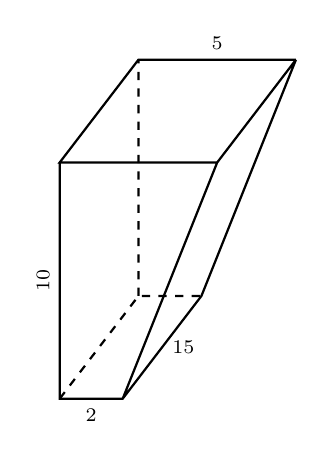
\begin{tikzpicture}[x={(1,0)},z={(0,1)},y={(.5,.87)},xscale=.4,yscale=.3]
\draw [thick] (0,0,0) -- node [above,rotate=90,pos=.5] {\scriptsize 10} (0,0,-10) --  node [below, pos=.5] {\scriptsize 2} (2,0,-10) -- node [right, pos=.5] {\scriptsize 15} (2,5,-10) -- (5,5,0)
							(5,5,0) -- (5,0,0)
							(5,0,0) -- (0,0,0) -- (0,5,0) --  node [above,pos=.5] {\scriptsize 5}(5,5,0)
							(5,0,0) -- (2,0,-10);						

\draw [thick,dashed] (0,0,-10) -- (0,5,-10) -- (2,5,-10)
																	(0,5,-10) -- (0,5,0);
\end{tikzpicture}\hfill\null

\item A conical water tank is 5 m deep with a top radius of 3 m. The tank is filled with pure water, with a mass density of 1000 kg/m$^3$. 
	\begin{enumerate}
	\item		Find the work performed in pumping all the water to the top of the tank.
	\item		Find the work performed in pumping the top 2.5 m of water to the top of the tank.
	\item		Find the work performed in pumping the top half of the water, by volume, to the top of the tank.
	\end{enumerate}

\item A water tank has the shape of a truncated cone, with dimensions given below, and is filled with water with a weight density of 62.4 lb/ft$^3$. Find the work performed in pumping all water to a point 1 ft above the top of the tank.\\

\hfill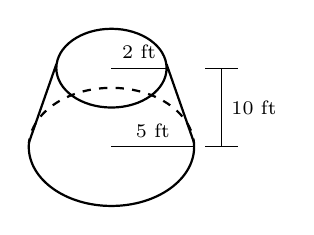
\begin{tikzpicture}[xscale=.7,yscale=.5]\draw [thick] (0,0) circle (1)
							(-1,.1) -- (-1.5,-1.9)
							(1,.1) -- (1.5,-1.9);
\draw (0,0)-- node [above,pos=.5] {\scriptsize 2 ft} (1,0)
			(0,-2) -- node [above,pos=.5] {\scriptsize 5 ft} (1.5,-2)
			(1.7,0) -- (2.3,0)
			(1.7,-2) -- (2.3,-2)
			(2,0) -- node [pos=.5,right] {\scriptsize 10 ft} (2,-2);
\draw [thick] (-1.5,-2) arc (180:360:1.5);
\draw [thick,dashed] (-1.5,-2) arc (180:0:1.5);
\end{tikzpicture}
\hfill\null

\item A water tank has the shape of an inverted pyramid, with dimensions given below, and is filled with water with a mass density of 1000 kg/m$^3$. Find the work performed in pumping all water to a point 5 m above the top of the tank.

\hfill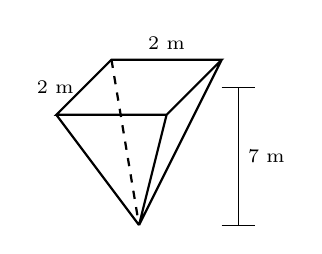
\begin{tikzpicture}[xscale=.7,yscale=.7]
\draw [thick] (0,0) -- node [pos=.5,left]{\scriptsize 2 m} (1,1) --node [above,pos=.5] {\scriptsize 2 m} (3,1) -- (2,0)--cycle
							(0,0) -- (1.5,-2)
							(3,1) -- (1.5,-2)
							(2,0) -- (1.5,-2);
\draw [thick,dashed] (1,1) -- (1.5,-2);
\draw (3,.5) -- (3.6,.5)
			(3,-2) -- (3.6,-2)
			(3.3,.5) -- node [pos=.5,right] {\scriptsize 7 m} (3.3,-2);
\end{tikzpicture}
\hfill\null

\item A water tank has the shape of an truncated, inverted pyramid, with dimensions given below, and is filled with water with a mass density of 1000 kg/m$^3$. Find the work performed in pumping all water to a point 1 m above the top of the tank.

\hfill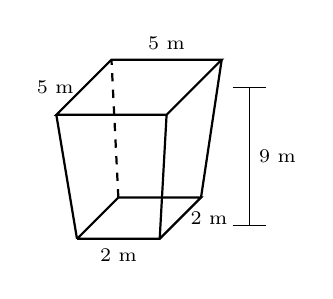
\begin{tikzpicture}[xscale=.7,yscale=.7]
\draw [thick] (0,0) node (A) {}-- node [pos=.5,left]{\scriptsize 5 m} (1,1)node (B) {} --node [above,pos=.5] {\scriptsize 5 m} (3,1) node (C) {} -- (2,0) node (D) {}--cycle;
\begin{scope}[scale=.75,shift={(.5,-3)}]
\draw [thick] (0,0) node (AA) {} -- (1,1) node (BB) {} -- (3,1) node (CC) {} -- node [right,pos=.5] {\scriptsize 2 m} (2,0) node (DD) {}-- node [pos=.5,below]{\scriptsize 2 m} (0,0);
\end{scope}
\draw [dashed,thick] (BB.center) -- (B.center);
\draw [thick] (AA.center) -- (A.center)
							(DD.center) -- (D.center)
							(CC.center) -- (C.center);
\draw (3.2,.5) -- (3.8,.5)
			(3.2,-2) -- (3.8,-2)
			(3.5,.5) -- node [pos=.5,right] {\scriptsize 9 m} (3.5,-2);\end{tikzpicture}
\hfill\null

%\item Consider the curve $f(x) = 3 \cos(\frac{x^3}{4})$ and the portion of its graph that lies in the first quadrant between the $y$-axis and the first positive value of $x$ for which $f(x) = 0$.  Let  $R$ denote the region bounded by this portion of $f$, the $x$-axis, and the $y$-axis.  Assume that $x$ and $y$ are each measured in feet.
%  	\ba
%		\item Picture the coordinate axes rotated 90 degrees clockwise so that the positive $x$-axis points straight down, and the positive $y$-axis points to the right.  Suppose that $R$ is rotated about the $x$ axis to form a solid of revolution, and we consider this solid as a storage tank.  Suppose that the resulting tank is filled to a depth of 1.5 feet with water weighing 62.4 pounds per cubic foot.  Find the amount of work required to lower the water in the tank until it is 0.5 feet deep, by pumping the water to the top of the tank.
%		\item Again picture the coordinate axes rotated 90 degrees clockwise so that the positive $x$-axis points straight down, and the positive $y$-axis points to the right.  Suppose that $R$, together with its reflection across the $x$-axis, forms one end of a storage tank that is 10 feet long.  Suppose that the resulting tank is filled completely with water weighing 62.4 pounds per cubic foot.  Find a formula for a function that tells the amount of work required to lower the water by $h$ feet.
%		\item Suppose that the tank described in (b) is completely filled with water.  Find the total force due to hydrostatic pressure exerted by the water on one end of the tank.
%	\ea 
  
\item A cylindrical tank, buried on its side, has radius 3 feet and length 10 feet.  It is filled completely with water whose weight density is 62.4 lbs/ft$^3$, and the top of the tank is two feet underground.
	\ba
		\item Set up an integral expression that represents the amount of work required to empty the top half of the water in the tank to a truck whose tank lies 4.5 feet above ground.
  
		\item With the tank now only half-full, set up an integral expression that represents the total force due to hydrostatic pressure against one end of the tank.
	\ea

\end{enumerate}

%---------------------------------------------
% END OF EXERCISES ON SECOND PAGE
%---------------------------------------------
\end{multicols*}
\end{adjustwidth*}

\afterexercises 

\cleardoublepage